\documentclass[a4paper,10pt]{article} 
\usepackage[francais]{babel}
\usepackage[utf8]{inputenc}
\usepackage[T1]{fontenc} 
%\usepackage{geometry}
\usepackage[a4paper, total={6in, 8in},top=1in]{geometry}
\usepackage{verbatim}
\usepackage{graphicx}
\usepackage{amsmath}
\usepackage{caption}

\title{RI Report}
\author{Jerémy Le - David Panou}

\begin{document}
\maketitle
\section{Introduction}

During our work, we have implemented and reviewed Structured classifier for different tasks including : Multi-class classification, hierarchical classification and ranking. As we would see, Structured models provide the ability to train a single model rather than training multiple binary classifiers.
The idea is to fit use the dual problem to fit a single classifier using multiple optimization problem of reduced size rather than several binary classifiers.

\section{MultiClass Kernel-based Vector Machines}

Several ways have been used to 
However, such models doesn't have the ability to capture the inter-class correlations since its break the multi-class correlation into independent binary problems.

The goal of Structured SVM is to

\section{Application to Information Retrieval and Computer Vision}

Structural SVM have been widely applied to Computer Vision 

\section{Structured SVM for MultiClassification}

We applied the Structured SVM classification to the usual task, obtaining the following loss curves : 


\begin{figure}
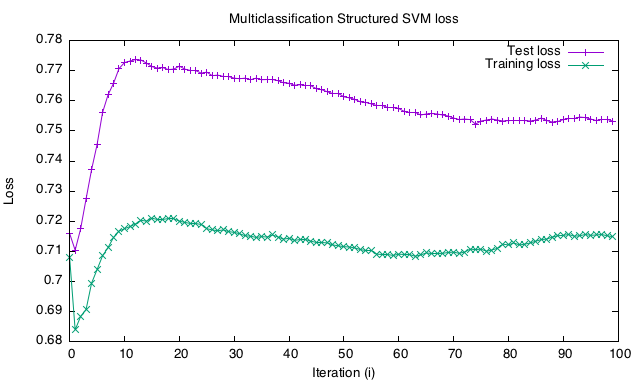
\includegraphics[width=0.5\linewidth]{pic/MultiClassification_Loss2}
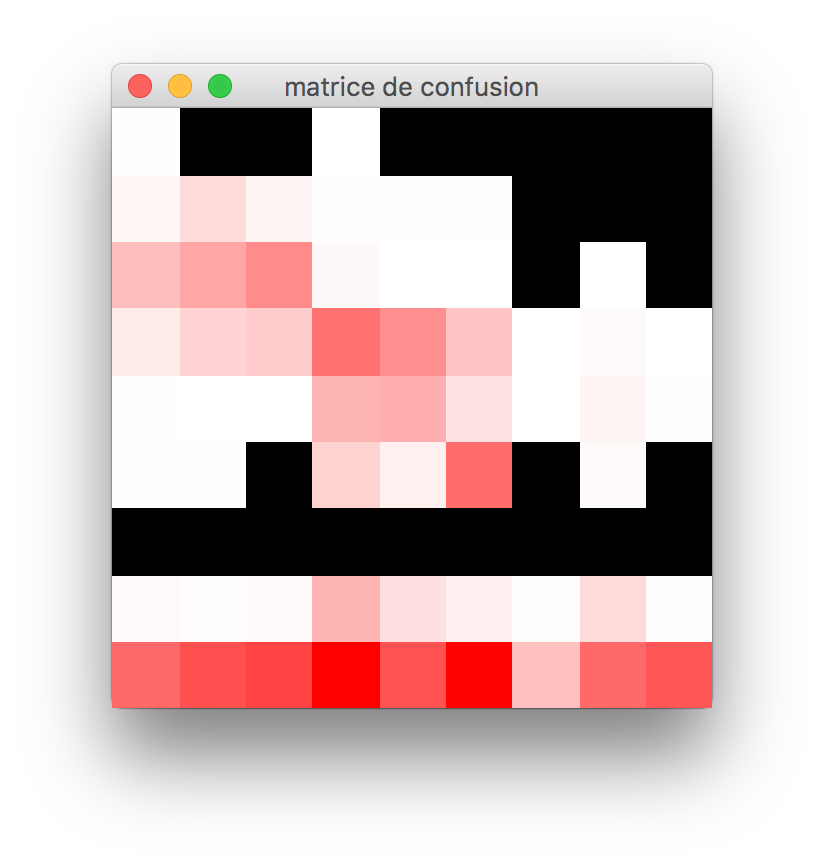
\includegraphics[width=0.5\linewidth]{pic/mc_cm}
\end{figure}
Corresponding to the following loss curves:


\begin{comment}
\column{.5\textwidth} % Right column and width
\begin{figure}
\includegraphics[width=0.8\linewidth]{pic/Momentum}
\end{figure}
Illustration taken from \cite{Duda}
\end{columns}
\end{frame}
\end{comment}


\medskip

\begin{thebibliography}{9}

\bibitem{}
Weston, J. and Watkins, C. (1999). Multiclass support vector machines, in
M. Verleysen (ed.), Proceedings of ESANN99, D. Facto Press, Brussels.

\end{thebibliography}


\end{document}
